\documentclass[conference]{IEEEtran}
\IEEEoverridecommandlockouts
\usepackage[utf8]{inputenc}
\usepackage[T1]{fontenc}
\usepackage[brazil]{babel}
\usepackage{cite}
\usepackage{amsmath,amssymb,amsfonts}
\usepackage{algorithmic}
\usepackage{graphicx}
\usepackage{textcomp}
\usepackage{xcolor}
\usepackage{booktabs}
\def\BibTeX{{\rm B\kern-.05em{\sc i\kern-.025em b}\kern-.08em
    T\kern-.1667em\lower.7ex\hbox{E}\kern-.125emX}}
\begin{document}

\title{Embeddings de not\'icias financeiras e comunicados do Copom em portugu\^es na previs\~ao do retorno di\'ario do Ibovespa: uma avalia\c{c}\~ao com valida\c{c}\~ao walk-forward}

\author{\IEEEauthorblockN{Hiago Lacerda}
\IEEEauthorblockA{\textit{Deep Learning} \\
\textit{Universidade Federal de Pernambuco - UFPE}\\
Recife, Brasil \\
hwal@cin.ufpe.br}
}

\maketitle

\begin{abstract}
Este trabalho avalia se embeddings textuais de not\'icias financeiras e o sinal de pol\'itica monet\'aria do Copom, ambos em l\'ingua portuguesa, melhoram a previs\~ao do retorno di\'ario (D+1) do Ibovespa, em compara\c{c}\~ao a baselines financeiros cl\'assicos (passeio aleat\'orio, ARIMA/ARIMAX) e a um modelo tabular treinado exclusivamente com dados de pre\c{c}o (XGBoost). Manchetes do InfoMoney (2018--2024, 57.611 manchetes) foram convertidas em representa\c{c}\~oes vetoriais por dois modelos de linguagem em portugu\^es -- BERTimbau e FinBERT-PT-BR -- e combinadas a uma rede LSTM de arquitetura parcimoniosa, treinada sobre vari\'aveis de pre\c{c}o. A valida\c{c}\~ao segue um protocolo walk-forward expans\'ivel, com embargo de 21 dias entre treino e teste, e todo ajuste dependente dos dados \'e realizado exclusivamente no conjunto de treino de cada fold. Nenhum modelo, de pre\c{c}o ou de texto, supera o acaso na previs\~ao da dire\c{c}\~ao do retorno de forma estatisticamente significativa (teste de Pesaran-Timmermann, $p>0{,}05$ ap\'os corre\c{c}\~ao de Holm em todos os casos). O sinal textual mostra-se reativo, e n\~ao preditivo: a polaridade de sentimento correlaciona-se fortemente com o retorno do mesmo dia ($r\approx0{,}20$), mas n\~ao com o retorno do dia seguinte ($r$ entre $0{,}00$ e $-0{,}04$). Testes de Diebold-Mariano indicam que um modelo tabular relativamente simples (XGBoost) \'e significativamente mais preciso do que diversas variantes de LSTM com texto, e que a inclus\~ao de sentimento textual piora a previs\~ao da LSTM de forma estatisticamente significativa. Sob custo de transa\c{c}\~ao de 5 pontos-base por opera\c{c}\~ao, dez das onze estrat\'egias mec\^anicas derivadas das previs\~oes apresentam \'indice de Sharpe negativo ou nulo, e a \'unica exce\c{c}\~ao observada \'e estatisticamente indistingu\'ivel de zero e inst\'avel entre folds. Conclui-se que, sob valida\c{c}\~ao rigorosa e sem vazamento temporal de informa\c{c}\~ao, embeddings de not\'icias financeiras em portugu\^es n\~ao melhoram a previs\~ao do retorno di\'ario do Ibovespa, constituindo resultado nulo obtido com rigor metodol\'ogico, e n\~ao uma limita\c{c}\~ao de implementa\c{c}\~ao.
\end{abstract}

\begin{IEEEkeywords}
previs\~ao de s\'eries financeiras, embeddings de texto, BERTimbau, FinBERT, valida\c{c}\~ao walk-forward, Ibovespa
\end{IEEEkeywords}

\section{Introdu\c{c}\~ao}

A hip\'otese de que not\'icias financeiras carregam informa\c{c}\~ao capaz de antecipar movimentos de pre\c{c}o \'e conhecida na literatura de finan\c{c}as e ganhou renovado interesse com o desenvolvimento de modelos de linguagem baseados em arquiteturas Transformer. Modelos como o BERT tornaram vi\'avel a extra\c{c}\~ao de representa\c{c}\~oes vetoriais densas a partir de texto em portugu\^es, superando a depend\^encia de l\'exicos de sentimento manualmente curados, e permitindo sua incorpora\c{c}\~ao a modelos de s\'eries temporais. Este trabalho investiga se embeddings textuais em portugu\^es, extra\'idos de not\'icias financeiras, melhoram a previs\~ao do retorno di\'ario (D+1) do Ibovespa em rela\c{c}\~ao a baselines financeiros cl\'assicos e a um modelo tabular robusto treinado exclusivamente com dados de pre\c{c}o.

O desenho experimental adota uma progress\~ao incremental de complexidade -- passeio aleat\'orio, ARIMA/ARIMAX, XGBoost, LSTM apenas com pre\c{c}o, e LSTM com embeddings textuais ou sinal do Copom --, na qual cada n\'ivel \'e validado isoladamente antes de ser adotado como refer\^encia para o n\'ivel seguinte. Essa progress\~ao responde a um prop\'osito metodol\'ogico espec\'ifico: caso a inclus\~ao de texto produza ganho real, este deve manifestar-se como melhora mensur\'avel e estatisticamente significativa sobre o melhor modelo de pre\c{c}o j\'a constru\'ido, e n\~ao como resultado favor\'avel obtido apenas em compara\c{c}\~ao com um baseline artificialmente fraco.

O alvo de todos os modelos \'e o log-retorno de D+1,
\begin{equation}
y_t = \ln\!\left(\frac{\text{close}_{t+1}}{\text{close}_t}\right),
\label{eq:target}
\end{equation}
avaliado sob tr\^es dimens\~oes: magnitude do erro (MAE, RMSE), acerto direcional (\emph{directional accuracy}, F1, MCC) e calibra\c{c}\~ao probabil\'istica (Brier Score). A valida\c{c}\~ao adota sempre o esquema walk-forward temporal, nunca parti\c{c}\~ao aleat\'oria, e toda transforma\c{c}\~ao dependente dos dados -- normaliza\c{c}\~ao, PCA, calibra\c{c}\~ao isot\^onica, sele\c{c}\~ao da ordem do modelo ARIMA -- \'e ajustada exclusivamente no conjunto de treino de cada fold.

As contribui\c{c}\~oes deste trabalho s\~ao as seguintes:

\begin{enumerate}
\item Um corpus de 57.611 manchetes do InfoMoney (2018--2024), coletado e temporalmente atribu\'ido a cada preg\~ao mediante corte expl\'icito \`as 17h (hor\'ario de fechamento da B3), respeitando o fuso hor\'ario hist\'orico, inclusive o hor\'ario de ver\~ao.
\item Uma compara\c{c}\~ao sim\'etrica entre dois modelos de linguagem em portugu\^es -- BERTimbau, de prop\'osito geral, e FinBERT-PT-BR, especializado em finan\c{c}as --, avaliando tanto seus embeddings quanto o sentimento expl\'icito produzido pelo FinBERT-PT-BR.
\item Evid\^encia direta, obtida por an\'alise de correla\c{c}\~ao contempor\^anea versus defasada, de que o sinal textual presente nas not\'icias financeiras \'e reativo, isto \'e, descreve o passado, e n\~ao preditivo, n\~ao antecipando o futuro.
\item Um protocolo de avalia\c{c}\~ao estat\'istica abrangente (Diebold-Mariano, Pesaran-Timmermann, corre\c{c}\~ao de Holm para m\'ultiplas compara\c{c}\~oes, avalia\c{c}\~ao multi-semente) aplicado uniformemente a 11 modelos, incluindo uma via adicional com comunicados do Copom, coletados via API de dados abertos do BCB e classificados por zero-shot.
\item Uma avalia\c{c}\~ao de custo de oportunidade financeiro (Sharpe, drawdown m\'aximo, custo de transa\c{c}\~ao) que demonstra que nenhum modelo produz vantagem econ\^omica estatisticamente robusta sob custos de transa\c{c}\~ao realistas, incluindo a an\'alise criteriosa do \'unico \'indice de Sharpe l\'iquido positivo observado, indistingu\'ivel de zero e inst\'avel entre folds.
\end{enumerate}

\section{Trabalhos Relacionados}

A literatura de previs\~ao de retornos financeiros com aprendizado profundo e dados textuais pode ser organizada em tr\^es frentes que orientam diretamente as escolhas metodol\'ogicas deste trabalho.

\textbf{Combina\c{c}\~ao de LSTM com embeddings financeiros.} Trabalhos recentes que combinam arquiteturas LSTM com representa\c{c}\~oes textuais de not\'icias financeiras \cite{gu2024finbertlstm} reportam ganhos modestos e inconsistentes entre mercados, frequentemente sem controle rigoroso de vazamento temporal na etapa de normaliza\c{c}\~ao ou sele\c{c}\~ao de vari\'aveis -- lacuna metodol\'ogica que este trabalho procura sanar ao exigir que todo ajuste estat\'istico (scaler, PCA, calibra\c{c}\~ao) ocorra exclusivamente dentro do treino de cada fold do walk-forward.

\textbf{Compara\c{c}\~oes de modelos de sentimento em finan\c{c}as.} Estudos comparativos sobre o uso de sentimento textual em previs\~ao financeira \cite{dahal2023comparative} documentam que o poder preditivo de sentimento agregado tende a ser pequeno e sens\'ivel \`a forma de agrega\c{c}\~ao temporal, o que refor\c{c}a a necessidade de uma regra de corte temporal expl\'icita e validada empiricamente -- adotada, neste trabalho, pela fun\c{c}\~ao \texttt{assign\_trading\_day}, com corte \`as 17h America/Sao\_Paulo, validada por su\'ite de testes automatizados (Se\c{c}\~ao \ref{sec:antivazamento}).

\textbf{FinBERT e modelos de linguagem especializados em finan\c{c}as.} A literatura de FinBERT \cite{araci2019finbert} estabelece que modelos de linguagem ajustados em corpora financeiros produzem sentimento mais alinhado ao dom\'inio do que modelos de sentimento gen\'ericos, mas n\~ao garante, por si s\'o, que esse sentimento seja \emph{preditivo}, apenas que constitui descri\c{c}\~ao mais \emph{precisa} do texto. Este trabalho distingue explicitamente essas duas propriedades (Se\c{c}\~ao \ref{sec:achado}): o FinBERT-PT-BR aqui utilizado produz sentimento fortemente correlacionado ao retorno \emph{contempor\^aneo}, mas n\~ao ao retorno \emph{futuro}, o que \'e consistente com a hip\'otese de efici\^encia informacional de mercado.

\section{Dados}

\subsection{Pre\c{c}os}
A s\'erie di\'aria do Ibovespa (\^{}BVSP), de julho de 2018 a dezembro de 2024, foi obtida junto ao Stooq. A s\'erie foi validada contra refer\^encias p\'ublicas conhecidas -- fundo da crise da COVID-19 em 23/03/2020 ($\approx$63.570 pontos) e fechamento do \'ultimo preg\~ao de 2024 ($\approx$120.283 pontos) --, com desvio de 0,00\% em ambos os casos. O per\'iodo de julho a dezembro de 2018 funciona como intervalo de aquecimento (\emph{buffer}) para vari\'aveis de janela longa. O per\'iodo de estudo compreende janeiro de 2019 a dezembro de 2024, totalizando 1.492 preg\~oes com alvo definido.

\subsection{Not\'icias}
Manchetes do InfoMoney, se\c{c}\~oes \emph{mercados} e \emph{economia}, referentes ao mesmo intervalo do buffer de pre\c{c}os, foram coletadas via sitemaps e extra\c{c}\~ao dos campos \texttt{datePublished}/\texttt{headline} do JSON-LD de cada p\'agina. Ap\'os deduplica\c{c}\~ao e nova tentativa de coleta dos registros com falha de rede, o corpus final totaliza 57.611 manchetes, cobrindo 100\% dos preg\~oes do per\'iodo de estudo.

Os timestamps do JSON-LD do InfoMoney foram verificados empiricamente como UTC verdadeiro, e n\~ao como deslocamento fixo pr\'e-aplicado. A convers\~ao para hora local emprega o m\'odulo \texttt{zoneinfo} com o fuso America/Sao\_Paulo, que trata corretamente o hor\'ario de ver\~ao hist\'orico, vigente no Brasil at\'e fevereiro de 2019, per\'iodo compreendido no intervalo de estudo. Uma implementa\c{c}\~ao que simplesmente subtra\'isse tr\^es horas fixas teria classificado incorretamente not\'icias publicadas durante o hor\'ario de ver\~ao.

A Fig.~\ref{fig:manchetes} ilustra a cobertura editorial, mostrando o volume di\'ario de manchetes ao longo do per\'iodo de estudo.

\begin{figure}[htbp]
\centerline{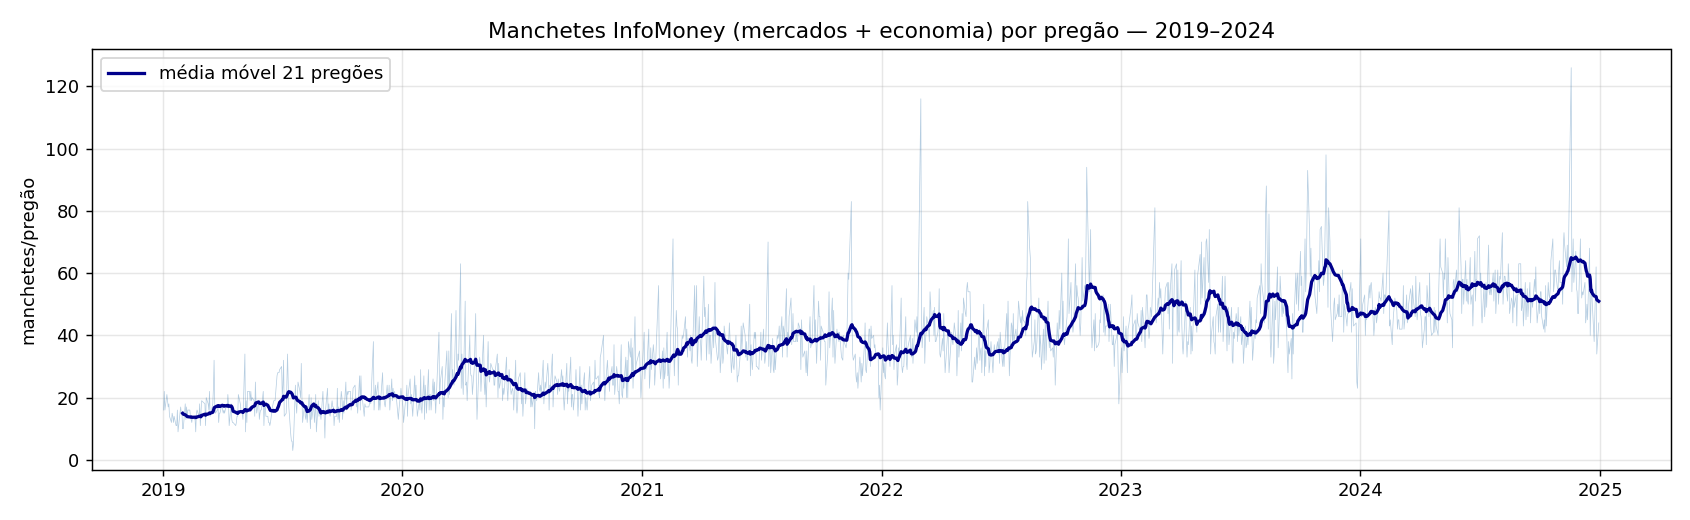
\includegraphics[width=0.48\textwidth]{manchetes_por_pregao.png}}
\caption{Manchetes coletadas por preg\~ao, 2019--2024.}
\label{fig:manchetes}
\end{figure}

\subsection{Alvo e corte temporal (anti-vazamento)}
\label{sec:antivazamento}

O alvo \'e gerado em um \'unico ponto do c\'odigo (\texttt{make\_target}), conforme a Eq.~\eqref{eq:target}, com o \'ultimo dia da s\'erie descartado por n\~ao possuir alvo definido. Cada not\'icia \'e atribu\'ida ao preg\~ao cujo fechamento ela pode informar por meio da fun\c{c}\~ao \texttt{assign\_trading\_day}, com corte inclusivo \`as 17h America/Sao\_Paulo: uma not\'icia publicada at\'e as 17h00, inclusive, do dia $D$ \'e atribu\'ida ao preg\~ao $D$; publicada depois, ao preg\~ao seguinte no calend\'ario da B3. Essa fun\c{c}\~ao \'e coberta por uma su\'ite de 14 testes automatizados (10 sobre o corte temporal), contemplando corte exatamente \`as 17h, transi\c{c}\~ao de sexta para segunda-feira, feriados, hor\'ario de ver\~ao hist\'orico e instantes UTC reais -- este \'ultimo desenhado para detectar o erro cl\'assico de tratar o fuso hor\'ario como deslocamento fixo, em vez de consultar a regra de hor\'ario de ver\~ao vigente na data.

\subsection{Comunicados do Copom}

Os 49 comunicados de decis\~ao de pol\'itica monet\'aria do Copom (reuni\~oes 219 a 267, dezembro de 2018 a dezembro de 2024) foram obtidos por meio da API p\'ublica de dados abertos do Banco Central (\texttt{dadosabertos.bcb.gov.br}), com texto integral e data de cada reuni\~ao. O comunicado \'e liberado no mesmo dia da decis\~ao, ap\'os o fechamento do preg\~ao ($\approx$18h30) -- tratado como publicado nesse hor\'ario e atribu\'ido ao preg\~ao seguinte pela mesma fun\c{c}\~ao \texttt{assign\_trading\_day} empregada para as not\'icias. A reuni\~ao 219 (dezembro de 2018), anterior ao per\'iodo de estudo, funciona como semente, de modo que os primeiros preg\~oes de 2019 n\~ao permane\c{c}am sem estado de pol\'itica monet\'aria conhecido.

\section{Metodologia}

\subsection{Vari\'aveis de pre\c{c}o}
\label{sec:features-preco}

O arquivo \texttt{features\_preco.parquet} cont\'em 18 vari\'aveis, todas calculadas com dados dispon\'iveis at\'e o dia $t$, inclusive, para prever $t+1$: retornos defasados (lags 0, 1, 2, 3, 5, 10), volatilidade realizada (janelas 5, 10, 21), momento/retorno acumulado (5, 10, 21), dist\^ancia \`a m\'edia m\'ovel (10, 21), calend\'ario (dia da semana, m\^es) e duas vari\'aveis de volume -- \texttt{vol\_rel} (volume relativo \`a m\'edia m\'ovel de 21 dias) e \texttt{dvol} (varia\c{c}\~ao logar\'itmica do volume). O n\'ivel absoluto de volume nunca \'e inclu\'ido, por carregar tend\^encia estrutural que constituiria sinal esp\'urio. A maior correla\c{c}\~ao absoluta entre uma vari\'avel e o alvo \'e 0,159, o que \'e consistente com aus\^encia de vazamento. O volume foi validado como sinal financeiramente plaus\'ivel antes de ser inclu\'ido: correla\c{c}\~ao entre retorno absoluto e volume de +0,18 (consistente com \cite{karpoff1987}) e persist\^encia estatisticamente significativa (Ljung-Box, $p\approx0$).

\subsection{Vari\'aveis de texto}

\textbf{BERTimbau} (\texttt{neuralmind/bert-base-portuguese-cased}): embeddings congelados (768 dimens\~oes), obtidos por mean-pooling mascarado por manchete e agregados por preg\~ao via m\'edia simples dos vetores do dia, acrescidos de \texttt{n\_noticias} e \texttt{emb\_dispersao} (dist\^ancia m\'edia ao centroide do dia).

\textbf{FinBERT-PT-BR} (\texttt{lucas-leme/FinBERT-PT-BR}): modelo \texttt{BertForSequenceClassification} ajustado para sentimento (positivo/negativo/neutro) em portugu\^es financeiro. A extra\c{c}\~ao ocorreu em uma \'unica passada, produzindo simultaneamente (i) as probabilidades de sentimento via forward oficial do classificador e (ii) os embeddings do codificador -- as duas vias pelas quais o modelo exp\~oe informa\c{c}\~ao, sem reconstru\c{c}\~ao manual da camada de classifica\c{c}\~ao. Os embeddings foram agregados por preg\~ao com a mesma metodologia do BERTimbau, resultando no mesmo formato e per\'iodo de estudo (1.492 preg\~oes, cobertura de 100\%).

Para redu\c{c}\~ao de dimensionalidade (768 $\to$ $k$), aplicou-se PCA ajustado \textbf{exclusivamente no treino de cada fold}, com dois valores de $k$: 8 (compress\~ao mais agressiva) e 30 (desambigua\c{c}\~ao). A vari\^ancia explicada difere consideravelmente entre as fontes: o BERTimbau ret\'em $\approx$45\% em $k=8$ e $\approx$69\% em $k=30$; o FinBERT-PT-BR, por tratar-se de modelo mais especializado, ret\'em $\approx$86\% em $k=8$ e $\approx$92\% em $k=30$ -- diferen\c{c}a estrutural que n\~ao se traduz em vantagem preditiva para nenhuma das duas fontes.

O sentimento expl\'icito do FinBERT-PT-BR foi agregado em quatro vari\'aveis densas por preg\~ao: \texttt{sent\_polaridade} (m\'edia de P(positivo) $-$ P(negativo) do dia), \texttt{sent\_dispersao}, \texttt{sent\_pos\_frac} e \texttt{sent\_neg\_frac}.

\subsection{Vari\'aveis do Copom}

Cada comunicado foi classificado por zero-shot (\texttt{MoritzLaurer/mDeBERTa-v3-base-mnli-xnli}, modelo de infer\^encia em linguagem natural multil\'ingue) entre dois r\'otulos -- vi\'es de aperto monet\'ario (\emph{hawkish}) versus afrouxamento (\emph{dovish}) --, gerando \texttt{copom\_hawkish\_score} $=P(\text{hawkish})-P(\text{dovish})\in[-1,1]$. Os comunicados possuem entre 1.219 e 1.876 tokens (mediana 1.482), o que excede, em todos os casos, o limite de 512 tokens do modelo, que trunca a entrada de forma silenciosa. Por essa raz\~ao, classificaram-se duas janelas textuais -- o in\'icio, correspondente ao truncamento natural do pipeline, e o trecho final (\'ultimos 1.500 caracteres, onde a decis\~ao costuma ser enunciada) --, selecionando-se a de maior correla\c{c}\~ao com a dire\c{c}\~ao real da decis\~ao: o in\'icio apresentou melhor desempenho ($r=+0{,}615$ contra $+0{,}424$ do trecho final, dilu\'ido por listas de votantes e texto de natureza burocr\'atica). Essa correla\c{c}\~ao de $+0{,}615$ entre o score e a dire\c{c}\~ao real da decis\~ao de Selic -- extra\'ida do t\'itulo oficial do comunicado, n\~ao pelo modelo -- confirma que o classificador zero-shot capta vi\'es real de pol\'itica monet\'aria, e n\~ao ru\'ido.

Como o regime de pol\'itica monet\'aria persiste entre reuni\~oes ($\approx$45 dias de intervalo m\'edio), o score, a dire\c{c}\~ao da \'ultima decis\~ao e o n\'umero de preg\~oes desde a \'ultima reuni\~ao s\~ao propagados por preenchimento antecedente (\emph{forward-fill}) di\'ario -- conven\c{c}\~ao padr\~ao em finan\c{c}as macroecon\^omicas, segundo a qual o mercado precifica o \'ultimo vi\'es conhecido do Banco Central at\'e a decis\~ao seguinte. O n\'ivel absoluto da Selic \'e \textbf{exclu\'ido} das vari\'aveis, pela mesma raz\~ao do volume (Se\c{c}\~ao~\ref{sec:features-preco}): carrega tend\^encia estrutural do ciclo econ\^omico, e n\~ao sinal de curto prazo.

\subsection{Modelos}

\begin{itemize}
\item \textbf{N\'ivel 1 -- Passeio aleat\'orio.} Regress\~ao: retorno previsto igual a zero. Dire\c{c}\~ao: persist\^encia. Probabilidade: frequ\^encia climatol\'ogica de alta no treino.
\item \textbf{N\'ivel 2 -- ARIMA/ARIMAX.} Ordem selecionada por AIC via \texttt{auto\_arima}, reajustada a cada fold, com $d=0$ justificado por teste ADF (estat\'istica $-11{,}86$, $p\approx7\times10^{-22}$). O diagn\'ostico de Ljung-Box indica estrutura linear fraca, por\'em significativa, no retorno, e estrutura mais forte no quadrado do retorno (\emph{clustering} de volatilidade). A valida\c{c}\~ao segue esquema walk-forward de um passo, reajustando o modelo a cada dia de teste. O ARIMAX emprega \texttt{n\_noticias} e \texttt{emb\_dispersao} como vari\'aveis ex\'ogenas, padronizadas por fold.
\item \textbf{N\'ivel 3 -- XGBoost.} \texttt{XGBRegressor} e \texttt{XGBClassifier} com hiperpar\^ametros conservadores e calibra\c{c}\~ao isot\^onica via hold-out temporal interno. Avaliado com $N=10$ sementes.
\item \textbf{N\'ivel 4 -- LSTM apenas com pre\c{c}o.} Arquitetura parcimoniosa (1 camada, 16 unidades ocultas, dropout 0,4), lookback de 21 dias, Adam, 75 \'epocas fixas, \texttt{StandardScaler} ajustado por fold. Avaliado com $N=5$ sementes; determinismo do PyTorch mantido fixo.
\item \textbf{N\'ivel 5 -- LSTM com texto ou Copom.} Id\^entico ao n\'ivel 4 em arquitetura, sementes, folds, calibra\c{c}\~ao e normaliza\c{c}\~ao; a \'unica diferen\c{c}a consiste na adi\c{c}\~ao das vari\'aveis textuais (ou do Copom, Via 3), isolando o efeito de cada fonte como a diferen\c{c}a entre essa variante e o n\'ivel 4.
\end{itemize}

Modelos com janela de lookback (LSTM) empregam \texttt{embargo=21} no walk-forward -- os primeiros 21 dias de cada bloco de teste s\~ao descartados. Baselines sem lookback empregam \texttt{embargo=0}. Ambos os grupos utilizam a mesma f\'ormula de particionamento, de modo que os limites de treino de cada fold coincidam exatamente entre fam\'ilias, tornando o teste da LSTM um subconjunto deslocado do teste do baseline no mesmo fold. Uma consequ\^encia dessa f\'ormula ($\text{fold\_size}=(n-\text{min\_train})/(n_{\text{splits}}+1)$) \'e que os \'ultimos 210 preg\~oes da s\'erie (mar\c{c}o a dezembro de 2024) n\~ao integram nenhum bloco de teste: a avalia\c{c}\~ao fora da amostra cobre janeiro de 2020 a fevereiro de 2024.

\subsection{Valida\c{c}\~ao estat\'istica}

\textbf{Pesaran-Timmermann} \cite{pesaran1992} avalia se a acur\'acia direcional de um modelo excede o valor esperado sob independ\^encia entre sinal previsto e sinal realizado, aplicado por modelo com os 5 folds concatenados.

\textbf{Diebold-Mariano} \cite{diebold1995}, com corre\c{c}\~ao de \textbf{Harvey-Leybourne-Newbold} \cite{harvey1997}, avalia se a acur\'acia de previs\~ao (erro quadr\'atico) de dois modelos difere significativamente:
\begin{equation}
DM = \frac{\bar{d}}{\sqrt{\mathrm{Var}(d)/n}}, \quad d_t = e_{1,t}^2 - e_{2,t}^2,
\label{eq:dm}
\end{equation}
ajustada pelo fator de pequena amostra $\sqrt{(n+1-2h+h(h-1)/n)/n}$ com $h=1$ e comparada \`a distribui\c{c}\~ao $t$-Student com $n-1$ graus de liberdade.

Tr\^es aspectos de protocolo merecem registro: (i) para modelos estoc\'asticos, os testes DM e os testes de rentabilidade simulada empregam a previs\~ao \emph{m\'edia entre as sementes}, constituindo pequeno ensemble, e n\~ao uma semente individual; (ii) a DA \'e calculada sobre o sinal da previs\~ao de regress\~ao, ao passo que F1, MCC e Brier utilizam a probabilidade calibrada com limiar 0,5, regras distintas que podem divergir em casos-limite; (iii) o calibrador isot\^onico \'e ajustado sobre as previs\~oes de um modelo treinado nos primeiros 80\% do treino e aplicado \`as previs\~oes do modelo treinado no treino completo -- aproxima\c{c}\~ao deliberada, adotada para n\~ao descartar 20\% dos dados de regress\~ao.

Duas fam\'ilias de compara\c{c}\~oes pareadas foram testadas: (i) LSTM apenas com pre\c{c}o em rela\c{c}\~ao a cada variante de texto/Copom, nos mesmos dias de teste; e (ii) XGBoost em rela\c{c}\~ao a cada variante de LSTM, na \textbf{interse\c{c}\~ao} dos dias de teste (185 de 206 dias por fold, em m\'edia). Os 13 $p$-valores resultantes foram corrigidos pelo m\'etodo de \textbf{Holm}.

\subsection{M\'etricas financeiras}

Adotou-se estrat\'egia mec\^anica long/short: a posi\c{c}\~ao no dia $t$ corresponde ao sinal da previs\~ao do modelo. O retorno l\'iquido di\'ario \'e dado por
\begin{equation}
r_t = \text{pos}_t \cdot y_t - c \cdot |\text{pos}_t - \text{pos}_{t-1}|,
\end{equation}
em que $c$ corresponde ao custo por unidade de turnover. Reportam-se o \'indice de Sharpe anualizado e o drawdown m\'aximo, sem custo (0 bps) e com custo de 5 pontos-base por opera\c{c}\~ao.

\section{Resultados}

\subsection{Diagn\'ostico de estrutura do retorno}

A Fig.~\ref{fig:acf} apresenta a autocorrela\c{c}\~ao do retorno e do retorno ao quadrado. O retorno exibe estrutura linear fraca; o retorno ao quadrado exibe \emph{clustering} de volatilidade consideravelmente mais pronunciado, evid\^encia de que a previsibilidade dispon\'ivel na s\'erie concentra-se, majoritariamente, na vari\^ancia, e n\~ao na dire\c{c}\~ao.

\begin{figure}[htbp]
\centerline{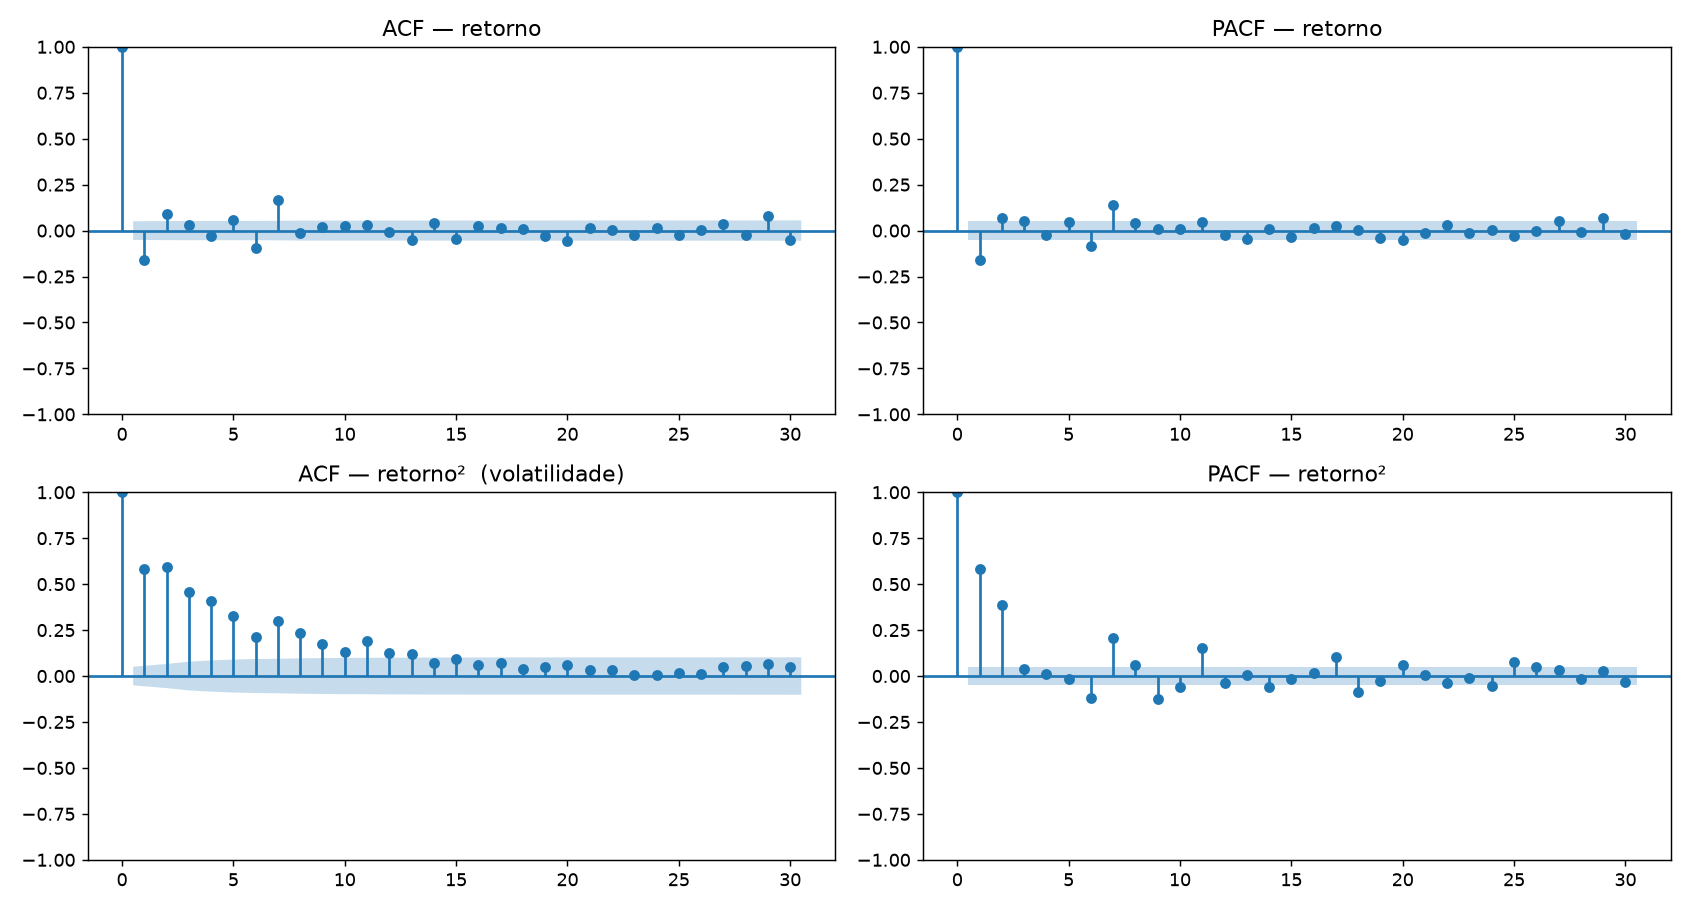
\includegraphics[width=0.48\textwidth]{acf_pacf_retorno.png}}
\caption{ACF/PACF do retorno di\'ario do Ibovespa.}
\label{fig:acf}
\end{figure}

\subsection{Tabela comparativa consolidada}

A Tabela~\ref{tab:comparativa} e a Fig.~\ref{fig:mcc} resumem os 11 modelos avaliados. Nenhum atinge signific\^ancia direcional a 5\% ap\'os corre\c{c}\~ao de Holm; o $p$-valor corrigido mais baixo corresponde ao XGBoost (0,577). A magnitude do MCC de todos os modelos situa-se tipicamente dentro de um desvio-padr\~ao entre sementes em rela\c{c}\~ao a zero, quando esse desvio est\'a dispon\'ivel, o que \'e vis\'ivel na Fig.~\ref{fig:mcc}, em que as barras de erro cruzam a linha de zero na pr\'atica totalidade dos modelos estoc\'asticos. Em termos de poder estat\'istico, com $n=1030$ observa\c{c}\~oes agregadas, o intervalo de 95\% para a DA de um classificador sem habilidade direcional \'e de $50\%\pm3{,}1$ p.p.; a maior DA observada (52,5\%, XGBoost) situa-se dentro dessa faixa. Os dados possuem poder para detectar habilidade direcional a partir de $\approx$53,1\%, patamar que nenhum modelo atinge.

\begin{figure*}[htbp]
\centerline{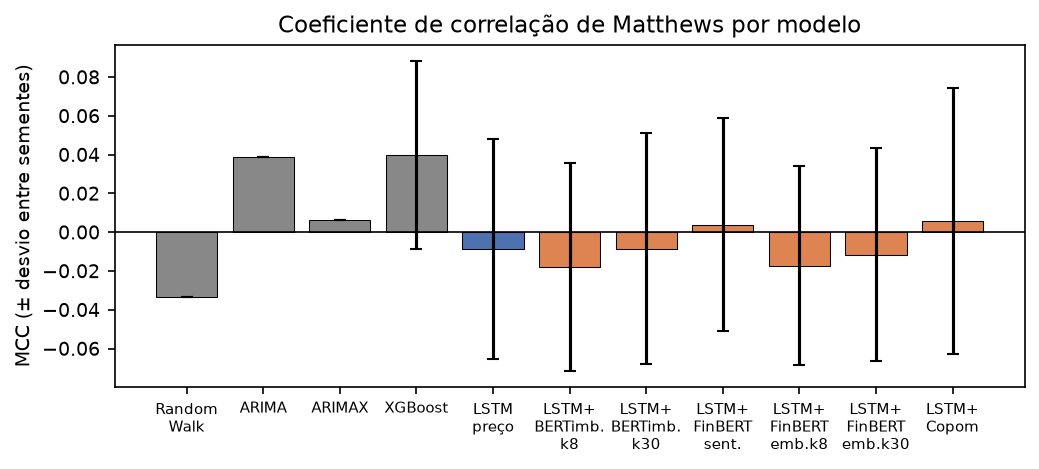
\includegraphics[width=0.85\textwidth]{fig_mcc_por_modelo.png}}
\caption{MCC por modelo, com barra de erro representando o desvio-padr\~ao entre sementes (quando aplic\'avel). Cinza: baselines determin\'isticos. Azul: LSTM apenas com pre\c{c}o. Laranja: variantes de LSTM com texto ou Copom.}
\label{fig:mcc}
\end{figure*}

\begin{table*}[htbp]
\caption{Tabela comparativa consolidada (fonte: \texttt{tabela\_comparativa\_final.csv})}
\begin{center}
\begin{tabular}{lccccccc}
\toprule
\textbf{Modelo} & \textbf{MAE} & \textbf{RMSE} & \textbf{DA} & \textbf{MCC} & \textbf{MCC ($\pm$dp)} & \textbf{Brier} & \textbf{PT $p$ (Holm)} \\
\midrule
Random Walk            & 0,0116 & 0,0159 & 0,485 & $-$0,033 & --      & 0,250 & 1,000 \\
ARIMA                   & 0,0120 & 0,0166 & 0,522 & $+$0,039 & --      & --    & 1,000 \\
ARIMAX (texto linear)   & 0,0124 & 0,0181 & 0,511 & $+$0,006 & --      & --    & 1,000 \\
XGBoost (pre\c{c}o)     & 0,0117 & 0,0161 & 0,515 & $+$0,040 & 0,049   & 0,266 & 0,577 \\
LSTM (pre\c{c}o)        & 0,0127 & 0,0172 & 0,494 & $-$0,009 & 0,057   & 0,273 & 1,000 \\
LSTM + BERTimbau $k$=8  & 0,0132 & 0,0181 & 0,494 & $-$0,018 & 0,054   & 0,273 & 1,000 \\
LSTM + BERTimbau $k$=30 & 0,0133 & 0,0178 & 0,508 & $-$0,009 & 0,060   & 0,265 & 1,000 \\
LSTM + FinBERT sent.    & 0,0136 & 0,0182 & 0,498 & $+$0,004 & 0,055   & 0,273 & 1,000 \\
LSTM + FinBERT emb. $k$=8  & 0,0136 & 0,0183 & 0,491 & $-$0,017 & 0,051 & 0,276 & 1,000 \\
LSTM + FinBERT emb. $k$=30 & 0,0131 & 0,0178 & 0,502 & $-$0,012 & 0,055 & 0,271 & 1,000 \\
LSTM + Copom            & 0,0140 & 0,0186 & 0,507 & $+$0,006 & 0,069   & 0,263 & 1,000 \\
\bottomrule
\end{tabular}
\label{tab:comparativa}
\end{center}
\end{table*}

\subsection{Testes pareados (Diebold-Mariano)}

Das 13 compara\c{c}\~oes pareadas testadas (6 do tipo LSTM-pre\c{c}o versus variantes de texto/Copom; 7 do tipo XGBoost versus variantes de LSTM), 4 permanecem significativas a 5\% ap\'os corre\c{c}\~ao de Holm (Tabela~\ref{tab:dm}). Em nenhuma das 13 compara\c{c}\~oes a adi\c{c}\~ao de texto ou Copom reduz o erro de forma significativa; nos casos em que h\'a signific\^ancia, esta aponta na dire\c{c}\~ao oposta. A compara\c{c}\~ao XGBoost versus LSTM+Copom situa-se pr\'oxima do limiar, sem contudo ultrapass\'a-lo ($p=0,055$ ap\'os Holm).

\begin{table}[htbp]
\caption{Compara\c{c}\~oes DM significativas ap\'os corre\c{c}\~ao de Holm}
\begin{center}
\begin{tabular}{lccc}
\toprule
\textbf{Compara\c{c}\~ao} & \textbf{DM} & \textbf{$p$ (Holm)} & \textbf{Dire\c{c}\~ao} \\
\midrule
pre\c{c}o vs.\ FinBERT-sent.     & $-3{,}12$ & 0,019 & texto piora \\
XGB vs.\ BERTimbau $k$=30    & $-3{,}52$ & 0,005 & XGB melhor \\
XGB vs.\ FinBERT-sent.       & $-3{,}90$ & 0,001 & XGB melhor \\
XGB vs.\ FinBERT emb.\ $k$=30 & $-3{,}18$ & 0,017 & XGB melhor \\
\bottomrule
\end{tabular}
\label{tab:dm}
\end{center}
\end{table}

Esse achado corrobora, com respaldo estat\'istico formal, um padr\~ao qualitativo j\'a observ\'avel na progress\~ao de complexidade: o aumento da sofistica\c{c}\~ao do modelo (RW $\to$ ARIMA $\to$ XGBoost $\to$ LSTM) n\~ao melhora a previs\~ao; em diversas compara\c{c}\~oes diretas, o modelo mais simples apresenta desempenho mensuravelmente superior.

Duas ressalvas de natureza metodol\'ogica s\~ao pertinentes a esses testes. Em primeiro lugar, a fam\'ilia de 13 compara\c{c}\~oes corrigida por Holm foi definida com base na estrutura do desenho experimental (n\'ivel 4 versus variantes de texto/Copom; XGBoost versus variantes de LSTM), e n\~ao registrada previamente -- a corre\c{c}\~ao protege contra infla\c{c}\~ao de falso-positivo \emph{dentro} dessa fam\'ilia, mas n\~ao contra o risco mais amplo de m\'ultiplas compara\c{c}\~oes n\~ao declaradas (\emph{garden of forking paths}), caso outras compara\c{c}\~oes tivessem sido exploradas antes da defini\c{c}\~ao dessas 13. Em segundo lugar, e de maior relev\^ancia: signific\^ancia estat\'istica n\~ao implica relev\^ancia econ\^omica. As diferen\c{c}as de erro quadr\'atico m\'edio subjacentes aos 4 resultados significativos da Tabela~\ref{tab:dm} ($\bar d$) s\~ao da ordem de $10^{-5}$, detect\'aveis em raz\~ao de $n\approx1030$ conferir poder estat\'istico para diferen\c{c}as de pequena magnitude, e n\~ao porque tais diferen\c{c}as sejam economicamente relevantes. A Se\c{c}\~ao~\ref{sec:financeiro-discussao} trata desse ponto diretamente: mesmo o modelo de melhor desempenho relativo apresenta \'indice de Sharpe l\'iquido pr\'oximo de zero ou negativo.

\subsection{Robustez: defasagem temporal e janela de lookback}
\label{sec:robustez}

Duas verifica\c{c}\~oes adicionais testam se o resultado nulo depende de escolhas arbitr\'arias de projeto. \textbf{Defasagem temporal (D versus D-1):} a substitui\c{c}\~ao do texto do pr\'oprio dia $D$ pelo texto do dia anterior ($D-1$) como vari\'avel do modelo LSTM+BERTimbau $k$=8 n\~ao altera o quadro geral -- MCC de $-0{,}016\pm0{,}054$ (texto $D-1$), valor intermedi\'ario entre o modelo apenas com pre\c{c}o ($-0{,}009$) e o texto do dia $D$ ($-0{,}018\pm0{,}054$), com a correla\c{c}\~ao preditiva texto($D-1)\to$retorno($D+1$) ainda mais pr\'oxima de zero do que a j\'a nula texto($D)\to$retorno($D+1$).

\textbf{Janela de lookback:} o n\'ivel 4/5 fixou lookback=21 dias. A Tabela~\ref{tab:lookback} apresenta o MCC para lookback $\in\{1,3,5,10,21\}$, tanto para o modelo apenas com pre\c{c}o quanto para o modelo com texto. Em nenhuma janela o MCC ultrapassa o intervalo de um desvio-padr\~ao entre sementes em torno de zero -- o resultado nulo n\~ao constitui artefato da escolha de 21 dias.

\begin{table}[htbp]
\caption{MCC por janela de lookback (embargo = lookback em cada linha)}
\begin{center}
\begin{tabular}{ccc}
\toprule
\textbf{Lookback} & \textbf{MCC s\'o-pre\c{c}o} & \textbf{MCC + BERTimbau $k$=8} \\
\midrule
1  & $-0{,}014\pm0{,}068$ & $+0{,}001\pm0{,}060$ \\
3  & $-0{,}006\pm0{,}042$ & $-0{,}021\pm0{,}053$ \\
5  & $-0{,}003\pm0{,}043$ & $-0{,}012\pm0{,}052$ \\
10 & $+0{,}005\pm0{,}045$ & $-0{,}006\pm0{,}055$ \\
21 & $-0{,}009\pm0{,}057$ & $-0{,}018\pm0{,}054$ \\
\bottomrule
\end{tabular}
\label{tab:lookback}
\end{center}
\end{table}

\subsection{Robustez: anisotropia dos embeddings e qualidade textual}
\label{sec:anisotropia}

Embeddings de BERT s\~ao conhecidamente anisotr\'opicos \cite{ethayarajh2019}: textos sem rela\c{c}\~ao sem\^antica tendem a exibir similaridade de cosseno bem acima de zero, pois parte substancial da vari\^ancia do espa\c{c}o vetorial concentra-se numa dire\c{c}\~ao gen\'erica compartilhada, n\~ao-informativa. Verificou-se empiricamente que a similaridade de cosseno m\'edia entre pares aleat\'orios de manchetes do corpus \'e $0{,}659$ (em um espa\c{c}o isotr\'opico, esperar-se-ia valor pr\'oximo de zero), confirmando anisotropia relevante. Como o pipeline principal aplica PCA diretamente sobre os embeddings crus, sem corre\c{c}\~ao pr\'evia, testou-se se essa anisotropia estaria suprimindo sinal preditivo real.

Aplicou-se \emph{whitening} (decorrela\c{c}\~ao e equaliza\c{c}\~ao de vari\^ancia entre dire\c{c}\~oes, ao molde de BERT-flow) sobre os embeddings crus antes da agrega\c{c}\~ao di\'aria e do PCA, de forma explorat\'oria (ajustado sobre a s\'erie completa, apenas para diagn\'ostico, sem uso em nenhum modelo reportado). Para o BERTimbau, o whitening eleva e estabiliza a correla\c{c}\~ao contempor\^anea (de $0{,}03$--$0{,}09$, vari\'avel conforme $k$, para $0{,}067$--$0{,}077$, est\'avel), indicando recupera\c{c}\~ao de sinal real antes diluído. Para o FinBERT, especializado em sentimento, a correla\c{c}\~ao contempor\^anea j\'a \'e alta e est\'avel mesmo nos embeddings crus ($0{,}215$, pr\'oxima da correla\c{c}\~ao de $+0{,}201$ j\'a obtida via a cabe\c{c}a de sentimento dedicada, Se\c{c}\~ao \ref{sec:achado}), n\~ao se beneficiando da corre\c{c}\~ao. Em ambas as fontes, contudo, a correla\c{c}\~ao \textbf{preditiva} permanece na faixa de ru\'ido para todo $k\in\{8,30,100,300\}$ testado (Tabela~\ref{tab:anisotropia}). Um teste de permuta\c{c}\~ao (500 repeti\c{c}\~oes, alvo embaralhado) confirma que o maior valor observado (BERTimbau whitened, $k=300$, $r=0{,}090$) \'e estatisticamente indistingu\'ivel de ru\'ido ($p=0{,}178$).

\begin{table}[htbp]
\caption{Correla\c{c}\~ao m\'axima ($|r|$) entre componentes e o alvo, cru vs.\ whitened ($k=300$)}
\begin{center}
\begin{tabular}{lcccc}
\toprule
\textbf{Fonte} & \multicolumn{2}{c}{\textbf{Preditivo}} & \multicolumn{2}{c}{\textbf{Contempor\^aneo}} \\
 & cru & whitened & cru & whitened \\
\midrule
BERTimbau & 0,085 & 0,090 & 0,088 & 0,068 \\
FinBERT   & 0,082 & 0,079 & 0,215 & 0,189 \\
\bottomrule
\end{tabular}
\label{tab:anisotropia}
\end{center}
\end{table}

Testaram-se ainda duas hip\'oteses sobre qualidade textual: (i) remo\c{c}\~ao de manchetes-template recorrentes (colunas fixas como ``Os 5 assuntos que v\~ao movimentar o mercado nesta [dia]'', 1,5\% do corpus, com embedding quase id\^entico a cada semana); e (ii) isolar manchetes de linguagem prospectiva (9,6\% do corpus) versus retrospectiva (0,4\%). Nenhuma altera\c{c}\~ao produziu correla\c{c}\~ao preditiva estatisticamente distingu\'ivel de ru\'ido (testes de permuta\c{c}\~ao, $p\in\{0{,}29$--$0{,}87\}$ em todos os casos). O resultado nulo mostra-se, portanto, robusto tanto \`a anisotropia dos embeddings quanto a interven\c{c}\~oes razo\'aveis de limpeza textual.

\subsection{Sentimento reativo versus sentimento preditivo}
\label{sec:achado}

A correla\c{c}\~ao entre o sentimento do FinBERT-PT-BR e o retorno depende substancialmente da dire\c{c}\~ao temporal considerada (Fig.~\ref{fig:sentimento}):
\begin{itemize}
\item Sentimento do dia $t$ em rela\c{c}\~ao ao retorno \textbf{contempor\^aneo} do dia $t$: $r=+0{,}201$
\item Sentimento do dia $t$ em rela\c{c}\~ao ao retorno de \textbf{D+1} (o alvo): $r=-0{,}039$
\end{itemize}

\begin{figure}[htbp]
\centerline{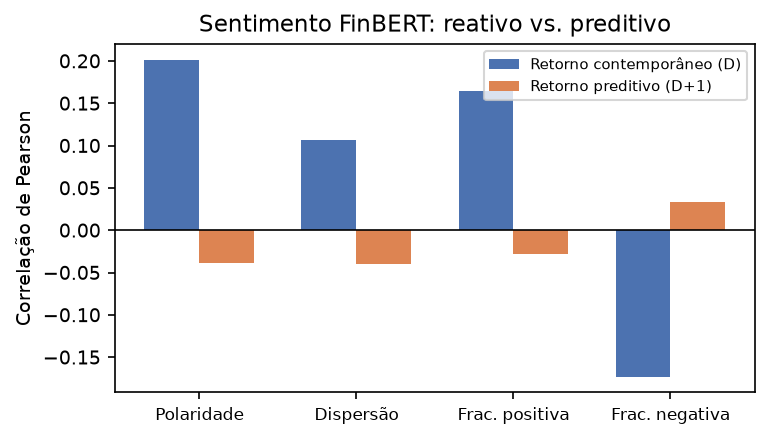
\includegraphics[width=0.48\textwidth]{fig_sentimento_reativo.png}}
\caption{Correla\c{c}\~ao das vari\'aveis de sentimento FinBERT com o retorno contempor\^aneo (D) versus o retorno preditivo (D+1, o alvo).}
\label{fig:sentimento}
\end{figure}

Todas as quatro vari\'aveis de sentimento agregado apresentam correla\c{c}\~ao preditiva entre $-0{,}04$ e $+0{,}03$ com o alvo, valores indistingu\'iveis de zero, ao passo que a correla\c{c}\~ao contempor\^anea de \texttt{sent\_polaridade} \'e aproximadamente cinco vezes maior em magnitude. Essa assimetria constitui a explica\c{c}\~ao de natureza mecan\'istica proposta neste trabalho para a aus\^encia de ganho preditivo do texto em todas as arquiteturas testadas: as not\'icias financeiras descrevem com fidelidade o que j\'a ocorreu no mercado no mesmo dia, mas n\~ao antecipam o que ocorrer\'a no dia seguinte, resultado consistente com a hip\'otese de efici\^encia informacional de mercado.

Cabe registrar uma limita\c{c}\~ao do FinBERT-PT-BR utilizado: o modelo exibe vi\'es para classifica\c{c}\~oes negativas (53\% das manchetes classificadas como negativas, contra 21\% como positivas, em per\'iodo de alta acumulada do \'indice). Esse vi\'es, contudo, n\~ao explica o resultado nulo: a correla\c{c}\~ao preditiva foi calculada sobre a polaridade cont\'inua, e n\~ao sobre a classe discreta, permanecendo estatisticamente nula.

\subsection{M\'etricas financeiras}
\label{sec:financeiro-discussao}

A Tabela~\ref{tab:financeiro} mostra que, sem custo de transa\c{c}\~ao, 5 dos 11 modelos exibem \'indice de Sharpe bruto positivo. Sob custo realista de 5 pontos-base por opera\c{c}\~ao, \textbf{dez dos onze modelos apresentam Sharpe negativo ou nulo}, inclusive o LSTM+BERTimbau $k$=30 (de $+0{,}175$ para $-0{,}019$). A \'unica exce\c{c}\~ao \'e o modelo LSTM+Copom (Sharpe l\'iquido $+0{,}42$), resultado que requer interpreta\c{c}\~ao criteriosa por tr\^es raz\~oes: (i) o retorno m\'edio di\'ario da estrat\'egia apresenta estat\'istica $t=0{,}86$ ($p\approx0{,}39$), sendo estatisticamente indistingu\'ivel de zero; (ii) o desempenho \'e inst\'avel entre folds (Sharpe por fold: $+0{,}84$, $+1{,}78$, $-1{,}69$, $+0{,}57$, $+0{,}18$; o terceiro fold perde 23,6\%); e (iii) trata-se do valor m\'aximo observado entre 11 estrat\'egias derivadas de modelos sem habilidade direcional detect\'avel (PT $p=0{,}27$ sem corre\c{c}\~ao; MCC $+0{,}006\pm0{,}069$), de modo que o m\'aximo de diversos modelos nulos tende a apresentar-se como positivo em decorr\^encia de efeito de sele\c{c}\~ao, e n\~ao de capacidade preditiva gen\'uina. N\~ao h\'a, portanto, evid\^encia de vantagem econ\^omica explor\'avel associada a esse resultado.

\begin{table*}[htbp]
\caption{M\'etricas financeiras (fonte: \texttt{metricas\_financeiras.csv}). Linha RW: a previs\~ao de regress\~ao \'e zero, logo a estrat\'egia nunca opera (piso trivial). Os per\'iodos de teste diferem levemente entre fam\'ilias, pois o embargo desloca os dias do LSTM; o buy-and-hold \'e calculado sobre o per\'iodo dos baselines. O drawdown m\'aximo das fam\'ilias LSTM atravessa os intervalos de embargo na concatena\c{c}\~ao dos folds.}
\begin{center}
\begin{tabular}{lcccc}
\toprule
\textbf{Modelo} & \textbf{Sharpe (0 bps)} & \textbf{Sharpe (5 bps)} & \textbf{MaxDD (5 bps)} & \textbf{N.\ trades} \\
\midrule
Buy-and-hold (refer\^encia) & 0,091 & --      & $-46{,}8\%$ & -- \\
Random Walk                & 0,000 & 0,000   & $0{,}0\%$   & 0 \\
ARIMA                      & $-0{,}035$ & $-0{,}445$ & $-45{,}2\%$ & 469 \\
ARIMAX                     & $+0{,}149$ & $-0{,}258$ & $-34{,}7\%$ & 467 \\
XGBoost                    & $+0{,}002$ & $-0{,}303$ & $-49{,}2\%$ & 350 \\
LSTM (pre\c{c}o)           & $-0{,}277$ & $-0{,}570$ & $-55{,}3\%$ & 335 \\
LSTM + BERTimbau $k$=8     & $-1{,}017$ & $-1{,}251$ & $-76{,}2\%$ & 267 \\
LSTM + BERTimbau $k$=30    & $\mathbf{+0{,}175}$ & $-0{,}019$ & $-41{,}1\%$ & 221 \\
LSTM + FinBERT sent.       & $-0{,}308$ & $-0{,}584$ & $-60{,}8\%$ & 316 \\
LSTM + FinBERT emb.\ $k$=8  & $+0{,}063$ & $-0{,}196$ & $-38{,}9\%$ & 296 \\
LSTM + FinBERT emb.\ $k$=30 & $-0{,}312$ & $-0{,}537$ & $-58{,}1\%$ & 258 \\
LSTM + Copom                & $+0{,}688$ & $+0{,}424$ & $-37{,}7\%$ & 301 \\
\bottomrule
\end{tabular}
\label{tab:financeiro}
\end{center}
\end{table*}

\begin{figure*}[htbp]
\centerline{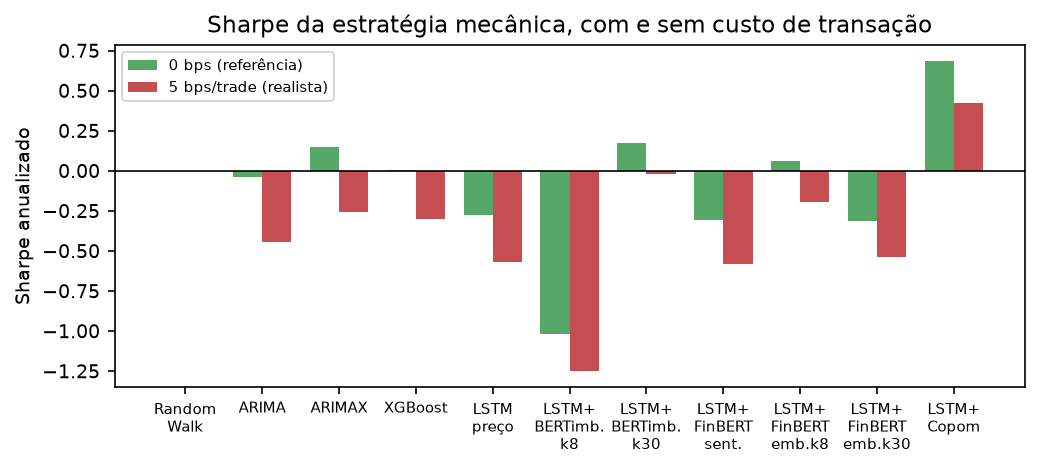
\includegraphics[width=0.85\textwidth]{fig_sharpe_custo.png}}
\caption{Sharpe anualizado por modelo, sem custo de transa\c{c}\~ao (0 bps) e com custo realista (5 bps/trade). Dez dos onze modelos ficam negativos ou pr\'oximos de zero sob custo; a exce\c{c}\~ao (LSTM+Copom) \'e estatisticamente indistingu\'ivel de zero e inst\'avel entre folds.}
\label{fig:sharpe}
\end{figure*}

O Random Walk, por nunca assumir posi\c{c}\~ao, constitui piso trivial de compara\c{c}\~ao. Esse conjunto de resultados corrobora, sob m\'etrica de utilidade econ\^omica direta, a conclus\~ao obtida pelos testes estat\'isticos de acur\'acia: nenhum modelo produz vantagem operacionaliz\'avel.

\section{Discuss\~ao}

Os resultados deste trabalho convergem para uma conclus\~ao consistente sob tr\^es perspectivas independentes -- acur\'acia estat\'istica de magnitude, habilidade direcional formal e utilidade econ\^omica: nenhum modelo, com ou sem texto, produz previs\~ao de retorno di\'ario do Ibovespa estatisticamente distingu\'ivel do acaso, uma vez aplicado o rigor estat\'istico apropriado.

O achado mais relevante n\~ao reside na aus\^encia de sinal em si, mas na \emph{explica\c{c}\~ao mecan\'istica} para essa aus\^encia (Se\c{c}\~ao \ref{sec:achado}): o texto financeiro em portugu\^es carrega sinal gen\'uino sobre o mercado, por\'em esse sinal \'e \textbf{contempor\^aneo}, n\~ao \textbf{preditivo}. Esse aspecto distingue este trabalho de resultados nulos n\~ao explicados e de trabalhos que reportam ganhos sem controle adequado de vazamento temporal, problema recorrente na literatura de FinBERT-LSTM discutida na Se\c{c}\~ao 2.

O sinal do Copom estende esse padr\~ao a uma fonte estruturalmente distinta do noticiário: trata-se de evento raro (49 reuni\~oes em 6 anos, contra 57.611 manchetes), de car\'ater oficial, cujo vi\'es \'e diretamente verific\'avel contra a decis\~ao real de Selic ($r=+0{,}615$). O classificador zero-shot mostra-se eficaz, mas o sinal de pol\'itica monet\'aria assim capturado tampouco antecipa o retorno de D+1 (MCC $+0{,}006\pm0{,}069$, Tabela~\ref{tab:comparativa}). Esse resultado sugere que a aus\^encia de ganho preditivo n\~ao constitui peculiaridade do noticiário do InfoMoney nem da extra\c{c}\~ao de sentimento, mas padr\~ao de car\'ater mais geral: informa\c{c}\~ao p\'ublica relevante, qualquer que seja sua fonte, parece j\'a estar precificada no fechamento do dia em que se torna conhecida.

O achado secund\'ario -- superioridade estatisticamente significativa do XGBoost em rela\c{c}\~ao a diversas variantes de LSTM -- requer interpreta\c{c}\~ao criteriosa: n\~ao significa que o XGBoost preveja o mercado, uma vez que seu MCC de $+0{,}040\pm0{,}049$ tamb\'em n\~ao \'e distingu\'ivel de zero. Significa, antes, que, entre modelos igualmente desprovidos de habilidade preditiva real, os mais simples produzem erros de magnitude menor e mais est\'avel -- argumento favor\'avel \`a pars\^imonia como princ\'ipio de projeto mesmo em cen\'arios nos quais nenhum modelo alcan\c{c}a sucesso preditivo.

Esses resultados devem ser interpretados \`a luz da hip\'otese de mercados eficientes: se o mercado brasileiro incorpora rapidamente informa\c{c}\~ao p\'ublica ao pre\c{c}o, o intervalo em que not\'icias financeiras poderiam ser exploradas por um modelo supervisionado, treinado com base no fechamento do dia anterior, tende a j\'a ter se encerrado no momento em que a not\'icia se torna texto indexado.

Um resultado adicional merece registro: o MCC do passeio aleat\'orio direcional (persist\^encia) \'e \emph{negativo} ($-0{,}033$), n\~ao pr\'oximo de zero. A correla\c{c}\~ao negativa entre persist\^encia e o retorno seguinte sugere leve revers\~ao \`a m\'edia de curt\'issimo prazo no Ibovespa di\'ario, padr\~ao que nenhum dos modelos testados, do ARIMA \`a LSTM, converteu em habilidade preditiva estatisticamente significativa (Tabela~\ref{tab:comparativa}). Esse resultado refor\c{c}a a leitura de efici\^encia informacional: ainda que exista estrutura fraca na s\'erie, tamb\'em observ\'avel no teste de Ljung-Box do retorno (Fig.~\ref{fig:acf}), tal estrutura n\~ao \'e suficientemente robusta para ser explorada de forma consistente por nenhuma das arquiteturas avaliadas.

\section{Limita\c{c}\~oes}

\begin{itemize}
\item \textbf{Frequ\^encia di\'aria.} O uso de fechamentos di\'arios pode subestimar a velocidade real de incorpora\c{c}\~ao de not\'icias ao pre\c{c}o.
\item \textbf{Vi\'es de classifica\c{c}\~ao do FinBERT-PT-BR.} Sobrerrepresenta\c{c}\~ao de sentimento negativo em per\'iodo de alta do \'indice, plausivelmente por interpretar vocabul\'ario t\'ecnico neutro como negativo; n\~ao mitigado, por restri\c{c}\~ao de tempo.
\item \textbf{Apenas o t\'itulo da mat\'eria, n\~ao o corpo.} Por desenho da coleta (requisi\c{c}\~ao em streaming, interrompida a $\approx$200KB para capturar somente o bloco JSON-LD do cabe\c{c}alho HTML, sem baixar a p\'agina completa), o corpus cont\'em exclusivamente a manchete de cada mat\'eria -- o corpo do texto nunca foi coletado. Isso subestima o conte\'udo informacional dispon\'ivel: a Se\c{c}\~ao~\ref{sec:anisotropia} identificou colunas-t\'itulo como ``Os 5 assuntos que v\~ao movimentar o mercado nesta [dia]'', cujo t\'itulo \'e gen\'erico por constru\c{c}\~ao, mas cujo corpo presumivelmente lista conte\'udo espec\'ifico do dia; o mesmo se aplica, em menor grau, a qualquer manchete como resumo compacto de um texto mais rico. N\~ao \'e poss\'ivel, com os dados aqui coletados, distinguir se a aus\^encia de sinal preditivo reflete a aus\^encia real de informa\c{c}\~ao explor\'avel nas not\'icias ou a perda de informa\c{c}\~ao inerente ao uso exclusivo de t\'itulos.
\item \textbf{Cobertura editorial \'unica.} O corpus est\'a restrito a um \'unico ve\'iculo (InfoMoney); vi\'eses editoriais espec\'ificos n\~ao foram comparados a outras fontes.
\item \textbf{Edi\c{c}\~ao de mat\'erias ap\'os a publica\c{c}\~ao original.} Verifica\c{c}\~ao direta no corpus (\texttt{datePublished} vs.\ \texttt{dateModified}) indicou que 4,3\% das mat\'erias foram editadas mais de 24h ap\'os a publica\c{c}\~ao original, e 2,6\% mais de 7 dias depois -- risco real, ainda que reduzido, de diverg\^encia entre o texto coletado e o texto publicado em tempo real.
\item \textbf{Redes sociais n\~ao implementadas.} O sinal de redes sociais (X/Twitter) n\~ao foi coletado nesta vers\~ao.
\item \textbf{Aus\^encia de baseline n\~ao recorrente.} N\~ao foi testado um MLP simples sobre a mesma janela achatada, o que impediria isolar se a recorr\^encia da LSTM, em si, agrega desempenho em rela\c{c}\~ao ao XGBoost.
\item \textbf{Componentes de PCA n\~ao interpretados.} O PCA \'e ajustado por fold, o que impede leitura est\'avel de quais dimens\~oes do embedding cada componente captura entre folds.
\item \textbf{Migra\c{c}\~ao de ambiente computacional.} Resultados originalmente produzidos em GPU T4 (Google Colab), reproduzidos localmente em RTX 3070 dentro da varia\c{c}\~ao esperada entre sementes, sem altera\c{c}\~ao de conclus\~oes qualitativas.
\item \textbf{Estrat\'egia financeira estilizada.} A avalia\c{c}\~ao de Sharpe/drawdown emprega estrat\'egia mec\^anica simples, sem dimensionamento de posi\c{c}\~ao, \emph{stop-loss} ou custo de financiamento.
\end{itemize}

\section{Conclus\~ao}

Sob protocolo de valida\c{c}\~ao walk-forward rigoroso -- com embargo temporal apropriado, ajuste de todo componente dependente de dados exclusivamente dentro do treino de cada fold, avalia\c{c}\~ao multi-semente e testes formais de signific\^ancia com corre\c{c}\~ao para m\'ultiplas compara\c{c}\~oes --, nenhum modelo testado neste trabalho, com ou sem embeddings de not\'icias financeiras em portugu\^es ou sinal de pol\'itica monet\'aria do Copom, prev\^e o retorno di\'ario do Ibovespa de forma estatisticamente distingu\'ivel do acaso. O sinal textual presente nas manchetes financeiras \'e gen\'uino, por\'em reativo: descreve o retorno do pr\'oprio dia com correla\c{c}\~ao de $+0{,}20$, e n\~ao o retorno do dia seguinte, cuja correla\c{c}\~ao com o sentimento \'e estatisticamente nula.

Trata-se de resultado nulo obtido com rigor metodol\'ogico, e n\~ao de limita\c{c}\~ao de implementa\c{c}\~ao. Demonstrar de forma controlada e reprodut\'ivel que um canal de informa\c{c}\~ao amplamente considerado \'util n\~ao produz vantagem preditiva mensur\'avel, e explicar \emph{por que} esse resultado ocorre, constitui, em si, contribui\c{c}\~ao cient\'ifica v\'alida.

\section*{Reprodutibilidade}
Todo o c\'odigo, dados brutos, vari\'aveis derivadas e resultados reportados neste trabalho est\~ao dispon\'iveis no reposit\'orio do projeto, com instru\c{c}\~oes de execu\c{c}\~ao em \texttt{README.md} e ambiente fixado em \texttt{requirements.txt}. A su\'ite de testes automatizados \texttt{test\_tcc\_utils.py} (14 casos, cobrindo corte temporal, hor\'ario de ver\~ao, embargo e gera\c{c}\~ao do alvo) documenta e verifica formalmente as garantias anti-vazamento descritas na Se\c{c}\~ao \ref{sec:antivazamento}.

\begin{thebibliography}{00}
\bibitem{araci2019finbert} D. Araci, ``FinBERT: Financial Sentiment Analysis with Pre-trained Language Models,'' \emph{arXiv preprint arXiv:1908.10063}, 2019.
\bibitem{diebold1995} F. X. Diebold and R. S. Mariano, ``Comparing Predictive Accuracy,'' \emph{Journal of Business \& Economic Statistics}, vol. 13, no. 3, pp. 253--263, 1995.
\bibitem{harvey1997} D. Harvey, S. Leybourne, and P. Newbold, ``Testing the Equality of Prediction Mean Squared Errors,'' \emph{International Journal of Forecasting}, vol. 13, no. 2, pp. 281--291, 1997.
\bibitem{karpoff1987} J. M. Karpoff, ``The Relation Between Price Changes and Trading Volume: A Survey,'' \emph{Journal of Financial and Quantitative Analysis}, vol. 22, no. 1, pp. 109--126, 1987.
\bibitem{pesaran1992} M. H. Pesaran and A. Timmermann, ``A Simple Nonparametric Test of Predictive Performance,'' \emph{Journal of Business \& Economic Statistics}, vol. 10, no. 4, pp. 461--465, 1992.
\bibitem{gu2024finbertlstm} W. Gu, Y. Zhong, S. Li, C. Wei, L. Dong, Z. Wang, and C. Yan, ``Predicting Stock Prices with FinBERT-LSTM: Integrating News Sentiment Analysis,'' in \emph{Proc. 8th Int. Conf. on Cloud and Big Data Computing (ICCBDC)}, Oxford, UK, 2024. DOI: 10.1145/3694860.3694870.
\bibitem{dahal2023comparative} K. R. Dahal, N. R. Pokhrel, S. Gaire, S. Mahatara, R. P. Joshi, A. Gupta, H. R. Banjade, and J. Joshi, ``A comparative study on effect of news sentiment on stock price prediction with deep learning architecture,'' \emph{PLOS ONE}, vol. 18, no. 4, e0284695, 2023.
\bibitem{ethayarajh2019} K. Ethayarajh, ``How Contextual are Contextualized Word Representations? Comparing the Geometry of BERT, ELMo, and GPT-2 Embeddings,'' in \emph{Proc. 2019 Conf. on Empirical Methods in Natural Language Processing and 9th Int. Joint Conf. on Natural Language Processing (EMNLP-IJCNLP)}, pp. 55--65, 2019.
\end{thebibliography}

\end{document}
